\documentclass{standalone}
\usepackage{tikz}
\usepackage{ctex,siunitx}
\setCJKmainfont{Noto Serif CJK SC}
\usepackage{tkz-euclide}
\usepackage{amsmath}
\usetikzlibrary{patterns, calc,3d}
\usetikzlibrary {decorations.pathmorphing,decorations.pathreplacing,decorations.shapes}
\begin{document}
\small
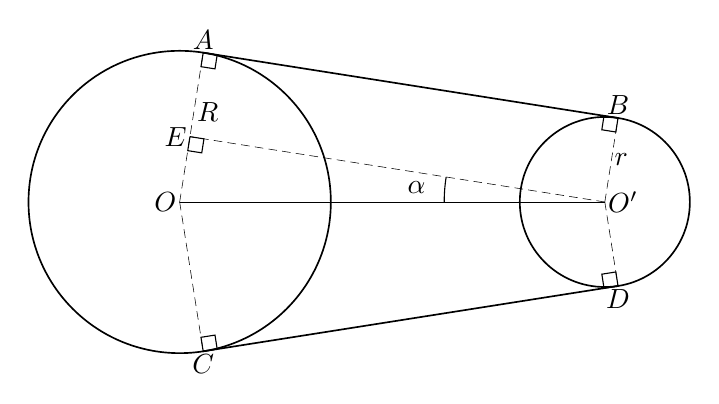
\begin{tikzpicture}[>=latex,scale=1.2,inner sep=1pt]
  \tkzDefPoints{0/0/O,4.5/0/O',1.6/0/R,5.4/0/r}
  \tkzDefSimilitudeCenter[ext](O,R)(O',r)\tkzGetPoint{I}
  \tkzDefLine[tangent from = I](O,R)\tkzGetPoints{C}{A}
  \tkzDefLine[tangent from = I](O',r)\tkzGetPoints{D}{B}
  \tkzDefPointsBy[projection=onto O--A](O'){E}
  \tkzDrawCircles[semithick,black](O,R O',r)
  \tkzDrawSegments[semithick](A,B C,D)
  \tkzDrawSegments(O,O')
  \tkzDrawSegments[densely dashed](O,A O',B O,C O',D O',E)
  \tkzLabelPoints[above](A,B)
  \tkzLabelPoints(C,D)
  \tkzLabelPoints[left](O,E)
  \tkzLabelPoints[right](O')
  \tkzMarkRightAngle[size=0.15](O,C,D)
  \tkzMarkRightAngle[size=0.15](O',D,C)
  \tkzMarkRightAngle[size=0.15](O,A,B)
  \tkzMarkRightAngle[size=0.15](O',B,A)
  \tkzMarkRightAngle[size=0.15](O',E,O)
  \tkzMarkAngle[size=1.7](E,O',O)
  \tkzLabelAngle[pos=2](E,O',O){$\alpha$}
  \tkzLabelLine[pos=0.5,right](O',B){$r$}
  \tkzLabelLine[pos=0.6,right](O,A){$R$}
\end{tikzpicture}
\end{document}